\section{Introduction}
\label{sec:intro}

In our recent paper~\cite{KobayashiPLDI2011}, we have shown how to
construct a fully-automated program verification tool (so called a
``software model checker'') for a tiny subset of functional language ML, a
simply-typed lambda calculus with recursion and integers.
The framework is an extension of higher-order model checker
(more precisely, the model checker for higher-order recursion scheme)
for infinite data domains such as integers by the techniques of
predicate abstraction and CEGAR.  This can be viewed as a higher-order
counterpart of previous software model checkers for imperative languages
like BLAST~\cite{Henzinger2002} and SLAM~\cite{Ball2002}.
We have implemented a verification tool, MoCHi, based on the framework.

The na\"{\i}ve application of the proposed approach, however, suffered
from scalability problems, both in terms of efficiency and supported
language features. For example, the previous framework does not support
recursive data structures and our implementation based on the framework
does not support control operations.  To explain the problem of the
previous framework/implementation, let us first review our previous
framework.

Our previous verification framework~\cite{KobayashiPLDI2011} is based on
predicate abstraction and CEGAR for a higher-order model checker.
Figure~\ref{fig:cegar} shows the overall structure of our previous
method.  First, an input program, written in a simply typed call-by-value
lambda calculus with recursion and integers, is abstracted to a
higher-order boolean program by predicate abstraction in Step 1.  The
abstracted program is verified by the higher-order model checker, where
models are described by higher-order recursion schemes, in Step 3.
Higher-order recursion schemes can be viewed as a simply typed
call-by-name lambda calculus with finite data domains and recursion.  To
resolve the gap between the evaluation strategies of higher-order
recursion schemes and higher-order boolean programs, we translate
call-by-value programs into call-by-name programs in Step 2. If the
abstracted program is safe, the source program is also safe.  If not, we
check whether the source program is in fact unsafe or the abstraction is too coarse
in Step 4. If the latter, we discover new predicates in Step 5.  We
repeat these steps until we find whether the program is safe or not.
%Our previous verification framework is a CEGAR-based one on higher-order
%model checker.  The verification proceeds as follows.  First, an input
%program, written in simply typed call-by-value lambda calculus with
%integers, is abstracted to a higher-order boolean program by predicate
%abstraction.  The abstracted program is verified by higher-order model
%checker. Higher-order model checker is the model checker for
%higher-order recursion schemes, it can be viewed as a simply typed
%call-by-name lambda calculus.  Here, to resolve the gap between
%semantics of higher-order recursion schemes and higher-order boolean
%programs, we need to translate call-by-value programs into call-by-name
%programs.  The abstracted program translated by CPS transformation is
%checked by the model checker. If the abstracted program is safe, the
%source program is also safe.  Otherwise, the model checker generates a
%counterexample for the abstracted program.  We can find a corresponding
%concrete error trace from the counterexample, and we can check whether
%the error path is feasible or not in the source program by symbolic
%execution.  If the error trace is feasible, the source program is
%unsafe.  Otherwise, the abstraction is too coarce to verify the source
%program.  We next discover new predicates to refute the
%counterexample, and repeat the above processes until we find out whether
%the program is safe or not.

\begin{figure}[tp]
 \begin{center}
  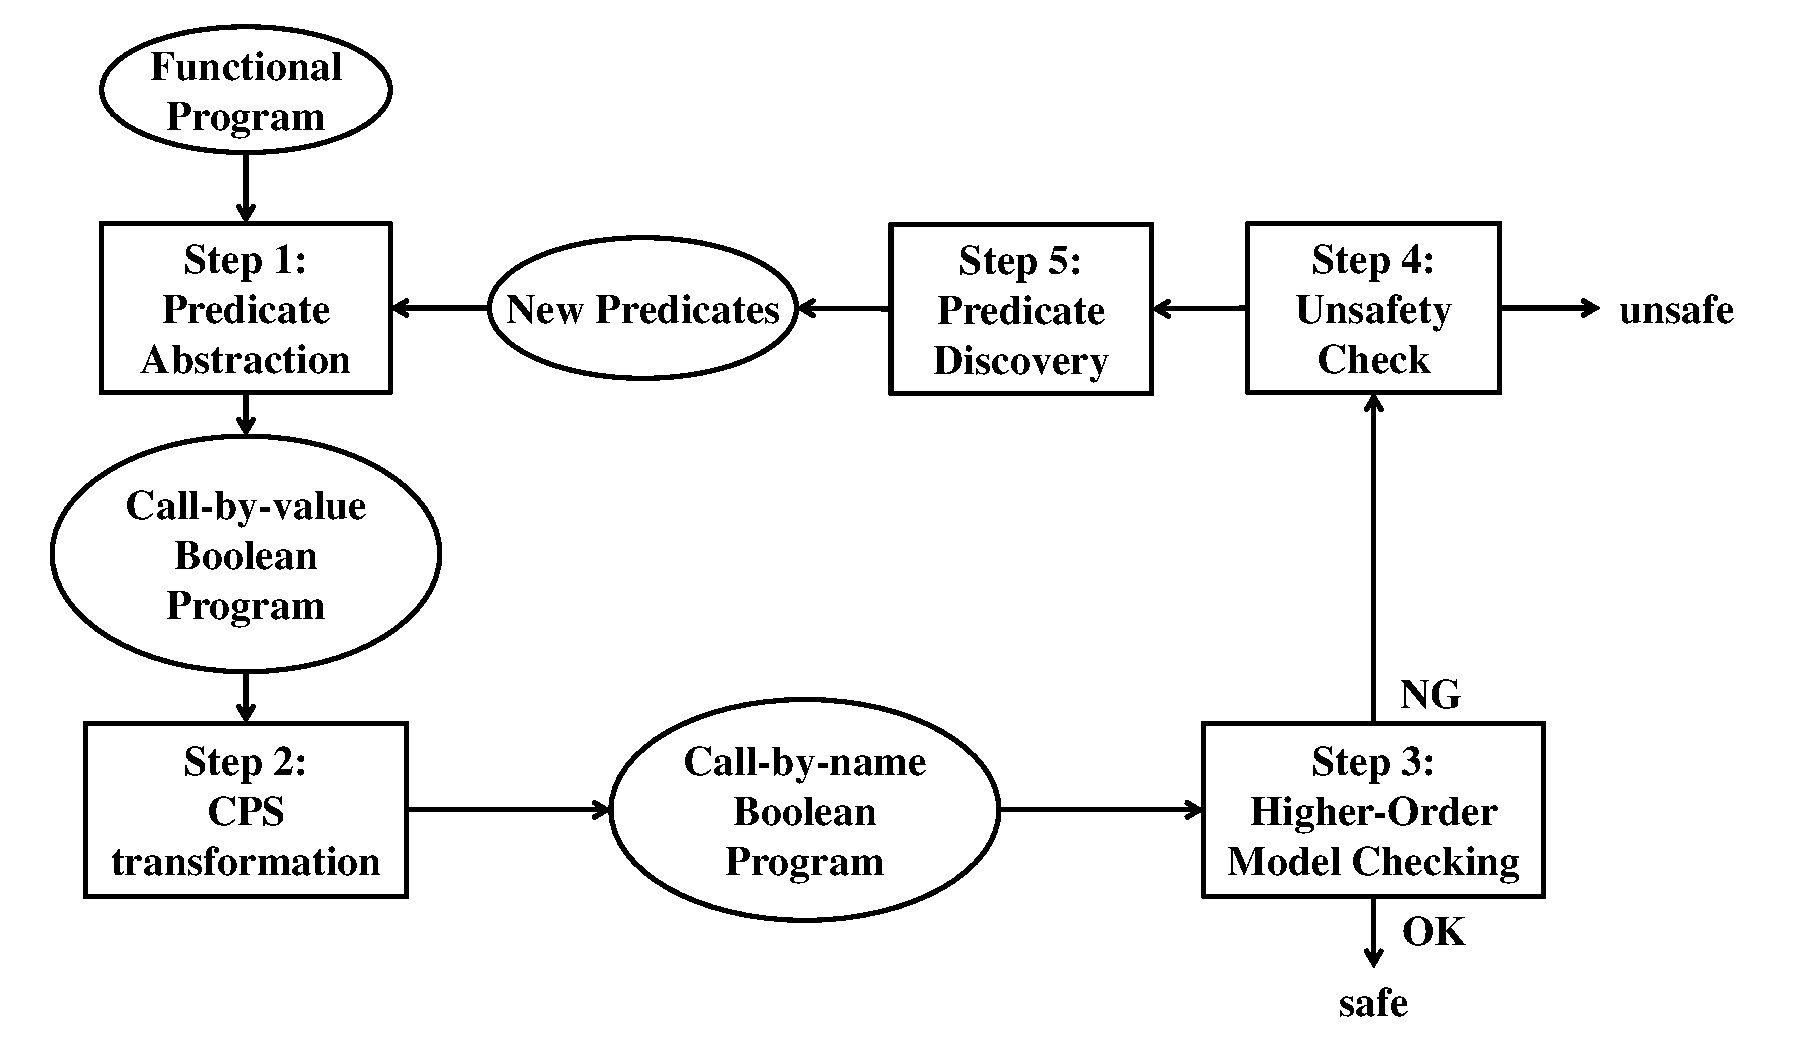
\includegraphics[scale=0.4]{overall.eps}
 \end{center}
\caption{Higher-Order Model Checking with Predicate Abstraction and CEGAR}
\label{fig:cegar}
\end{figure}

%The na\"{\i}ve application of the proposed approach, however, suffered
%from scalability problems, both in terms of efficiency and supported
%language features.  The verification framework supports infinite data
%domains other than integers.  However, we need interpolant theorem
%provers that can deal with the each infinite data domains (e.g., lists
%and trees).  Moreover, the verification framework does not support
%control operations (e.g., exceptions and call/cc).

%The na\"{\i}ve application of the proposed approach, however, suffered
%from scalability problems, both in terms of efficiency and supported
%language features.
%In this paper, we address the following
%problems of our previous work.
%\begin{enumerate}
% \item The previous framework requires an appropriate set of predicates for all
%       functions in the source program of predicate abstraction.
% \item Na\"{\i}ve CPS transformation extremely increases the computational cost
%       of model checking of higher-order boolean program because of the
%       increase of the order of the program.
% \item The previous framework does not support recursive data
%       structures like lists and trees.  Moreover, the previous
%       implementation does not support control operations like
%       exceptions and call/cc.
%\end{enumerate}
%
%We discuss each problem in more detail and explain our approach below.

In this paper, we address three problems of our previous work.
We discuss each problem and explain our approach below.

\begin{enumerate}
\item The main bottleneck of the previous version of MoCHi was the
      predicate abstraction and discovery (Steps 1 and 5), rather than
      higher-order model checking. Our previous method for predicate
      abstraction tried to abstract every integer argument of a function
      to a tuple of booleans. As a result, verification of a program did
      not succeed until an appropriate set of predicates is found for
      \emph{every} function in the program.  For example, consider the
      program shown in Fig.~\ref{fig:sum}.  The program can be successfully
      verified if we abstract the program by using predicates
      $\Abs{y}{y \geq 0}$ for the second argument of \texttt{add} and
      $\Abs{r}{r \geq x}$ for the return value of \texttt{add} and
      \texttt{sum}.  The following is the
      abstracted program using the above predicates.

\begin{figure}[t]
\begin{alltt}
let add x y = x + y
let rec sum x = if x <= 0 then 0 else add x (sum (x-1))
let main x = assert (sum x >= x)
\end{alltt}
\caption{Example Program for Selective Predicate Abstraction}
\label{fig:sum}
\end{figure}
\begin{alltt}
let add () by = if by then true else rand_bool()
let rec sum () = if rand_bool() then true
                else add (if sum () then true else *)
let main x = assert (sum ())
\end{alltt}
      Here, \texttt{rand\us{}bool()} means a non-deterministic boolean
      value.  \texttt{by} denotes whether $\mathtt{x} \geq 0$ or not.
      Automatically finding all such appropriate predicates is
      difficult.  In the previous paper~\cite{KobayashiPLDI2011}, we
      have adapted CEGAR to find such predicates, but the technique is
      necessarily heuristic, and often fails.  If we abstract the
      program using only the predicate $\Abs{r}{r \geq x}$ for the return
      value of \texttt{sum}, we get the following abstracted program.
\begin{alltt}
let add () () = ()
let rec sum u = if rand_bool() then true
                else let b = sum () and u = add () () in
                       rand_bool()
let main x = assert (sum ())
\end{alltt}
      Since the return value of \texttt{add} is non-informative, the
      abstraction is too coarse.

      To reduce the burden to the program discovery phase, we introduce
      a refinement of predicate abstraction called \emph{selective
      predicate abstraction}.  As the name suggests, the selective
      predicate abstraction applies predicate abstraction to only a
      certain set of functions, and avoids abstraction of the other
      functions by inlining them.  The selective predicate abstraction
      generates the following safe program by using only the
      predicate $\Abs{r}{r \geq x}$ for the return values of \texttt{sum}
      and inlining \texttt{add}.
\begin{alltt}
let rec sum () = if * then true else if sum () then true else *
let main () = assert (sum ())
\end{alltt}
      In this way the selective predicate abstraction improves the
      precision of abstraction and reduce the cycle of CEGAR.

%%The first problem increases the number of CEGAR-cycle.
%To see the first problem, consider the following program.
%\begin{alltt}
%let add x y = x + y
%let rec sum x = if x < 0 then 0 else add x (sum (x-1))
%let main x = assert (sum x >= 0)
%\end{alltt}
%In our previous framework, we have to give predicate $\Abs{x}{x\geq0}$
%for return values of \texttt{sum}, return values of \texttt{add}, and
%arguments of \texttt{add}.  The following is the abstracted program
%using the predicate.
%\begin{alltt}
%let add bx by = if bx \&\& by then true else rand_bool()
%let rec sum _ = if rand_bool() then true
%                else add true (sum ())
%let main x = assert (sum ())
%\end{alltt}
%Here, \texttt{bx} is true and \texttt{bx} is true denote that
%$\mathtt{x} \geq 0$ and $\mathtt{y} \geq 0$, respectively.
%%If we abstract the program using predicate
%%$\Abs{x}{x\geq0}$ for return values of function \texttt{sum}, we get the
%%following abstracted program.
%%\begin{alltt}
%%let add u1 u2 = ()
%%let rec sum u = if rand_bool() then true
%%                else let b = sum () in
%%                     let u = add () () in
%%                       rand_bool()
%%let main x = assert (sum ())
%%\end{alltt}
%\texttt{rand\us{}bool()} means a non-deterministic boolean value.
%In fact, we can abstract the source program to the following program by
%using the definition of \texttt{add} with predicate $\Abs{x}{x\geq0}$
%only for return values of \texttt{sum}.
%\begin{alltt}
%let rec sum _ = if rand_bool() then true
%                else if sum () then true else rand_bool()
%let main x = assert (sum ())
%\end{alltt}
%In the body of \texttt{sum}, \texttt{add x (sum (x-1))}, i.e. \texttt{x
%+ sum (x-1)}, is abstracted to \texttt{if sum () then true else rand\us{}bool()}
%because $\mathtt{sum ()}$ is true denotes $\mathtt{sum (x-1)} \geq 0$.
%The case of $\mathtt{b}=\mathtt{false}$ is similar.
%We distinguish functions that are abstracted from functions that is not abstracted.
%In the example above, functions \texttt{sum} and \texttt{main} are abstracted, and
%function \texttt{add} is not abstracted.
%We abstract programs, intuitively, with extracting functions which is not abstracted.
%We formalize this abstraction, called selective predicate abstraction.

\item Another efficiency problem is caused by CPS transformation.  As
      stated above, our approach needs CPS transformation to resolve the
      gap between the evaluation strategies of higher-order recursion schemes and
      higher-order boolean programs.  However, CPS transformation increases the
      order\footnote{The order of program $t$ is the maximum order of
      the types of functions in $t$.  The order of type $\tau$ is
      defined by $\mathit{order}(\INT)=0$,
      $\mathit{order}(\TFun{\tau_1}{\tau_2}) =
      \mathit{max}(\mathit{order}(\tau_1)+1, \mathit{order}(\tau_2))$.}
      of programs and the growth of the order is not bounded by a constant.
      Since the complexity of model checking of higher-order recursion
      scheme is $n$-EXPTIME complete for order-$n$ recursion scheme, the
      increase of the order of an input is crucial to the verification
      time.
%
      For example, consider the following program.
\begin{alltt}
let rec check x f = f x; check (x+1) f
let f x = assert (x >= 0)
let main n = check n f
\end{alltt}
%Function \texttt{check} may cause an assertion failure only when two arguments are given.
      The above program is translated into the following program by
      a na\"{\i}ve call-by-value CPS transformation~\cite{Plotkin1975}.
\begin{alltt}
let rec check x k1 = k1 (\(\lambda\)f.\(\lambda\)k2.f x (\(\lambda\)_.check (x+1) (\(\lambda\)g.g f k2)))
let f x k = assert (x >= 0); k ()
let main n k = check n (\(\lambda\)g. g f k)
\end{alltt}
      To preserve the evaluation order of an original call-by-value program,
      each function of the translated call-by-name program takes
      a continuation and passes its return value to the continuation.  Note here that the
      order of the translated program is increased to 5.
%\begin{alltt}
%let check x k1 = k1 (\(\lambda\)y.\(\lambda\)k2. assert (x = y); k2 ())
%let main k = check (\(\lambda\)f. f n k)
%\end{alltt}
%let apply x k1 = k1 (\(\lambda\)f.\(\lambda\)k2. f x k2)
%let check x k1 = k1 (\(\lambda\)y.\(\lambda\)k2. assert (x = y); k2 ())
%let main n k = check n (\(\lambda\)f1. apply n (\(\lambda\)f2. f2 f1 k))
      We can, however, obtain the following order-3 program by omitting the continuation \texttt{k1} of \texttt{check},
      which is actually unnecessary since a partial application of \texttt{check} in the original program never causes side effects including an assertion failure,
\begin{alltt}
let rec check x f k = f x (\(\lambda\)_.check (x+1) f k)
let f x k = assert (x >= 0); k ()
let main n k = check n f k
\end{alltt}
%This transformation uses the fact that the application to the first
%argument does not cause an assertion failure and the context of
%\texttt{call n} is not required to have a continuation.
      Our CPS transformation avoids such unnecessary insertions of
      continuations.  We formalize this transformation, called
      \emph{selective CPS transformation}.

%Higher-order model checking (more precisely, the model
%checking of higher-order recursion schemes) has been studied
%recently~\cite{Ong2006}, and applied to verification of higher-order
%functional programs~\cite{KobayashiPOPL2009,KobayashiPLDI2011}.  Our
%previous framework~\cite{KobayashiPLDI2011} can verify higher-order
%programs.  The framework, however, cannot deal with recursive data
%structures, which are necessary for practical functional languages.
%Moreover, the na\"{\i}ve implementation based on the framework cannot
%verify large programs.
%
%In this paper, we introduce extensions and optimizations of the
%verification framework.  The extensions are language extensions to deal
%with recursive data structures (e.g., lists and trees) and control
%operators (e.g., exceptions and call/cc).  Our approach is to translate
%a source program written in the extended language to a program written
%in the previous language. This translation is sound and complete.

%The goal of the verification is to check
%that all assertions in a program never fail and pattern matching
%failures do not occur.

%\memo{The problem of the previous predicate abstraction}
%we introduce selective predicate abstraction as an optimization technique
%
%\memo{The problem of the previous model checking}
%we introduce selective CPS transformation as an optimization technique
%
%\memo{for language extension}
%(iii) functional encoding of recursive data structures and control operations to support a larger subset of ML.

\item The third problem is the insufficiency of supported language
      features.  The framework proposed in our previous work requires an
      automated interpolating theorem prover for predicate abstraction and
      discovery, but practical provers are not available for recursive data
      structures like lists and trees. Thus, the implementation dealt with
      only integers as infinite data domains.
      
      To support recursive data structures without relying on interpolating
      theorem provers for recursive data structures, we extend our verification framework as follows.
      As a preprocessing of our CEGAR-based model checking,
      we translate programs that manipulate recursive data structures into ones that manipulate only integers.
      The transformation is carried out by encoding recursive data structures using higher-order functions.  For example, a list is
      encoded to a function that maps an index $i$ to the $i$-th element.
      In a similar way, we support control operations (e.g., exceptions and call/cc) by using higher-order functions.
\end{enumerate}

%Our contributions are (i) the formalization of selective predicate
%abstraction using a simple but effective way to overcome the first
%efficiency problem, (ii) the formalization of selective CPS
%transformation to overcome the efficiency second problem, (iii) the
%formalization for language extension for recursive data structures
%(e.g., lists and trees) and control operations (e.g., exceptions and
%call/cc) that is sound, complete, and general for verification
%frameworks for higher-order language, and (iv) the implementation and
%experiments.

The rest of this paper is organized as follows. 
%In Sect.~\ref{sec:model-check}, we introduce our previous framework for
%higher-order programs with integers, which is the base of our framework
%described in this paper.
We first formalize the source language of verification in
Sect.~\ref{sec:language}.  Section~\ref{sec:opt} formalizes the
selective predicate abstraction and the selective CPS transformation.
Section~\ref{sec:extension} shows the language extensions for recursive
data structures and control operations.  Section~\ref{sec:experiments}
reports experiments.  Section~\ref{sec:related} discusses related work
and Sect.~\ref{sec:conclusion} concludes the paper.














%\section{Introduction}
%\label{sec:intro}
%[background]
%
%In this paper, we propose the verification method for program with
%recursive data types and control operator.  The goal of the verification
%is to check that a program does not execute the command \texttt{fail}.  We can
%also check that pattern matching failures and uncaught exceptions do not
%occur by a trivial transformation. For example, a program
%\texttt{(match t with ...)} cause a pattern match failure if and only if 
%a program \texttt{(match t with ... | \_ -> fail)} execute \texttt{fail}.
%
%The base of our framework is the verification of higher-order programs with integers.
%
%The idea of this framework is to translate a target program (with
%recursive data structures and exceptions) to a higher-order program with
%integers.  For example, the lists $[2;3;5]$ is encoded to a pair of the length $3$
%and a function $f$ such that $f(1)$, $f(2)$, $f(3)$ returns $2$, $3$,
%$5$, respectively.
%A function which takes lists and/or returns lists is encoded to
%a higher-order function which takes functions and/or returns functions.
%
%[Show running example of verifying a program with lists.]
%
%[discovering general predicates]
%
%[Show running example of discovering general predicates.]
%
%
%[the overview of this framework]
%
%We formalize the verification method for a language with lists.
%The verification for recursive data structures are argue in the Section ...
%
%The rest of this paper is organized as follows. We first formalize the
%target language in Section~\ref{sec:target-language}.  In
%Section~\ref{sec:model-check}, we introduce our previous framework for
%higher-order program with integers, which is the base of our framework
%described in this paper.  Section~\ref{sec:encoding} shows the program
%transformation which generate a program without lists from a program with lists,
%and argue about recursive data structures.
%Section~\ref{sec:control} shows that how to deal with control operators.
%Section~\ref{sec:discover}.
%Section~\ref{sec:experiments} reports preliminary experiments.
%Section~\ref{sec:related} discusses related work and
%Section~\ref{sec:conclusion} concludes the paper.
%
